\documentclass[oneside, astronomy, noacknowlegments]{BYUPhys}

% Your name
  \Author{Scott Leland Crossen}

% Enter the date your thesis is approved
  \Year{[Year]}
  \Month{[Approval Month]}

% If you have a long title, split it between multiple lines using the \\ command
  \Title{Optically Detected Magnetic Resonance;
Computational Predictions\\and Experimental Results
  }

% Your research advisor
\AdvisorTitle{Advisor}
  \Advisor{Dr. John S. Colton}

% For honors theses, enter the name of the honors Representative
  \HonorsRepresentative{Kristine Hansen}

% The text of your abstract
  \Abstract{ [The abstract is a summary of the thesis/dissertation
  with emphasis on the findings of the study. The abstract must not
  exceed 350 words in length and fit on one page, single spaced.] }

 \Keywords{[A comma-separated list of descriptive words for search purposes]}

% Acknowledge those who helped and supported you
  \Acknowledgments{
    [Acknowledgements should be simple, in good taste, and fit on one page]
  }

%% The members of your committee (masters only need A and B, PhD need all 4)
%  \MemberA{Committee Member A}
%  \MemberB{Committee Member B}
%  \MemberC{Committee Member C}
%  \MemberD{Committee Member D}
%

\begin{document}

 % Start page counting in roman numerals
 \frontmatter

 % This command makes the formal preliminary pages.
 % You can comment it out during the drafting process if you want to save paper.
 \makepreliminarypages

 % Make the table of contents.
 \tableofcontents

 % Start regular page counting at page 1
 \mainmatter

 % Include a list of figures
 \listoffigures 










\chapter{Introduction}

\section{Qualitative Description of ESR and ODMR}
\label{sec:qualitative}

\textit{Optically Detected Magnetic Resonance} (ODMR) is a particular form of \textit{Electron Paramagnetic Resonance} (EPR) which is more commonly known as \textit{Electron Spin Resonance} (ESR). The latter two of these terms (EPR and ESR) are synonymous; The former (ODMR) is a particular subset of ESR that utilizes a luminescence measuring technique as a means to collect ESR information. In literature, it is common to see both of these terms followed by the designation "spectroscopy" which signifies that they are tools to study properties of matter via electromagnetic radiation. Though the extent of their application has grown over the years, ESR and ODMR are most commonly used to study the spin-properties of electrons and electron-holes trapped in metal lattices. They can be used to study free radicals in organic materials and are also important in studying the local environment of lattice defects through a technique using angular-dependent ODMR. One particular use of ODMR is the study of electron-spin coherence via a technique known as \textit{Electron Spin Echo}. This can be useful when studying what properties and conditions lead to superior state coherence for qubit candidate materials in quantum computing.

The intellectual foundation of Electron Spin Resonance is rooted in Quantum Mechanics. Bound electrons in matter have discrete and quantized energy levels that govern what frequencies of light are emitted when transitions between energy levels are made. For electron systems, which are fermions and thus subject to the Pauli exclusion principle, the energy levels are 2nd order degenerate when bound in matter. In Quantum Mechanics we choose to describe this degeneracy in terms of spins: we say an electron is either "spin-up" or "spin-down". Each energy level can have at most two electrons of opposite spins inhabiting it (and thus the degeneracy). The spin terminology is arbitrary however, and is really just an attempt at comparing electrons to particles. In truth, electron spin is a term for a property that is emergent from solving the wave equation. However, it nonetheless describes the principle of conservation of momentum that would be found in classical system such as a top and so the term makes sense and has persisted in usage today. In this case, the electron’s spin is a description of the magnetic moment for when the particle is in the presence of a magnetic field. In the case of electrons bound in matter within an magnetic field, the energy levels of the molecule will split according to the "Zeeman Effect" and the spin-states of the electrons can be observed - most commonly through a photoluminescence or other fluorescence measuring technique.

The Zeeman effect itself is crucial in understanding the principles of ESR. In the presence of a magnetic field, populations of free electrons will form a spin-1/2 system between a higher-energy "spin-up" state and a lower-energy "spin-down" state. In matter, different parities of spin-states can be formed between the interactions of different energy levels with different transition selection rules. A spin-1/2 system in the presence of a magnetic field is shown in \ref{fig:Zeeman}. As seen here, the energy levels of the two differing spins diverge linearly for an increasing magnetic field. The difference in energy between these two levels is typically in the microwave frequency domain. For a given magnetic-field strength there will be a set of characteristic microwave frequencies that the electrons are most prone to emitting when transitioning between these quantized states. In a spin-1/2 system there will only be one frequency for a given magnetic field corresponding to the difference between the two zeeman lines at the given field strength. Likewise, for a given microwave target signal, there will be a variety of magnetic field strengths which are most adept at transitioning bound electrons between states. This unique pairing between both the microwave frequency and magnetic field strength is the resonant condition that ESR is based off of and also the means that it uses to discover information about materials.

\begin{figure}
    \caption[Zeeman effect and resonant conditions in matter]{\label{fig:Zeeman}
     Zeeman effect for a two level system showing spin energy levels as a function of applied magnetic field. For arbitrary field strength the energy difference is shown as a function of $\mu$, $g$, and the field strength $B$.}
\end{figure}

\section{The Defect Nature of Materials}

\section{Electron Spin, Quantum Computing, and Qubits}

Classical Computation is almost always based off of a binary system. In these architectures, the computer's register, memory, and general logical states are either in a logical 'true' or a logical 'false' state. A 'true' state corresponds to a high voltage and a 'false' state corresponds to a grounded voltage. A computer's bits can be in either of these two states - 1 or 0 - but not both.

A spin-1/2 system also describes a binary system between a higher-energy basis state and a lower-energy basis state. In this comparison, the spin-1/2 system will be measured (and the wave function collapsed) to be in either of these two states - but not both. The important difference between the the spin-1/2 system and the classical computer bit model is that the spin system can have states that exist as linear combinations of the two basis up/down states. In accordance with Quantum Mechanics, this means that the spin-1/2 system can exist as a superposition between both the spin-up and spin-down states and has a certain probability of being measured in each. It is important to note that this superposition does not mean that the state exists as some value in between an excited state and a lower state. Rather, it exists as both states simultaneously.

Because of this unique property of spin systems, they can then be used as the basis for forming what is called a "quantum computer". Though it largely depends on the architecture, Quantum computers can be thought of to manipulate information in a similar fashion to that of a classical computer. Both have logical operators and storage bits and both are algorithmically based. Quantum computers, however, utilize this unique possibility of superposition to make probabilistic calculations for many different states at the same time. This happens through the quantum mechanical operators that initialize and manipulate the states which are stored in "qubits" - or the quantum computer's version of classical bits that can exist in these superposition types of states. Because of the existing theoretical construction from nondeterministic finite automata to deterministic finite automata, quantum computers are also turing complete in the broad definition of that term.

Today, there is large emphasis within the scientific community in building viable, scalable quantum computers. The reason for this is that quantum computers offer reduced computational time limits for certain types of algorithms. Certainly however, these machines are not necessarily more adept at common tasks such as processing videos to be scrubbed by common users, but are rather designed to carry out a few types of intense calculations in logarithmic time that would normally have a polynomial time dependence. The most notable use for quantum computers in our modern society is within the field of computer security and encryption. Quantum computers have the ability to compute prime factors via Shor's algorithm in a much faster time than traditional computers. This ability would essentially render all of the current RSA encryption methods obsolete in addition to anything that relies on public/private key encryption such as bitcoin.

Although more than just spin systems can be used as the all-important qubits for quantum computing, we will focus on this type - specifically spin-1/2 systems formed from electrons - for the basis of our discussion. As mentioned earlier, Electron Spin Resonance is the major tool used to study the spin properties of materials. In the case of quantum computation, ESR is used to study possible qubit materials that might eventually be used in such machines. Currently, one of the major difficulties in creating quantum computers is finding materials that can form superposition states that remain coherent (and reliable) over prolonged periods of time. In order to understand what properties of materials lead to superior qubit construction and state coherence, ESR can be used in conjunction with electron spin echo experiments to study the coherence of electrons in a spin-1/2 system. Moreover, ESR can be used alone to study the spin system itself and the local environment of the defects in matter that form them. Knowledge of this important topic will serve to increase our ability to construct better qubits for use in quantum computers.

\section{Previous Work (Our Research Group and Others)}

\subsection{Preliminary Work and Results}

The work performed in this thesis references in large part the work done by Kyle Miller and Jacob Embley - two students who worked under Dr. John Colton and have since graduated from BYU. Their work was mostly performed on the topic of Electron Spin Coherence in Proton-Irradiated Silicon Carbide and is documented in their senior theses both of related titles. This thesis, however, will not be on the same topic as the former two but will expand on one aspect used by both of these two students in their work - ODMR. In addition, both Embley and Miller used a particular species of SiC which is one of the two principal materials of investigation in this thesis.

Appendix \ref{chpt:AppendC} includes a publication that Embley, Colton, Miller, Myself and a few others produced on the topic of spin coherence in proton irradiated silicon carbide. It has been accepted by \textit{Physical Review B} and will appear in publication later in the year 2017. This publication serves as a capstone to the work of both Embley and Miller as included in their senior theses and will serve as the context for which this thesis was produced.

In addition to the work done by Miller and Embley, an additional study was performed on a similar material of the SiC specimen which is not included in either the aforementioned theses or publication. This project is included in Appendix \ref{chpt:AppendA}. The major difference with Appendix \ref{chpt:AppendA} and the theses produced by Miller and Embley is the fluence of irradiation used on the SiC sample in question. Miller's work was primarily concerned with a $10^{14}$ $cm^{-2}$ proton-irradiated sample of SiC. Embley likewise worked with a $10^{13}$ $cm^{-2}$ proton-irradiated sample of SiC. In Appendix \ref{chpt:AppendA} I work with a $10^{17}$ $cm^{-2}$ electron-irradiated sample of SiC in much the same way as used by Embley. With this additional sample, a more comprehensive analysis and additional results are presented.

\subsection{Experimental Setup}

The experimental setup used for the majority of this thesis was set up and tested by Kyle Miller and Jacob Embley. Miller initially set up all the necessary instrumentation to be used in his experiment which is detailed in his thesis. Later, Embley improved upon most of Miller's design and achieved increased precision and improved results. The experiment used by both Embley and Miller was eventually repurposed and slightly modified for the experiment detailed in this thesis. A full summary and implementation of the experimental setup can be found in \ref{sec:Experiment}. This section includes both the setup used by Miller and Embley as well as the modified components used by myself.

\subsection{Samples and Collaborative Efforts}

The work done for this thesis was done in collaboration with two groups of people. Firstly, the silicon carbide samples used were produced and partially characterized by Dr. Sam Carter of the Naval Research Lab. These samples were irradiated with different fluences of particles in order to introduce different concentrations of defects into the material. It was Carter's work that ultimately led us to obtain such high quality samples for optical characterization and electron spin resonance studies.

The second collaborative group that we worked with was Dr. Mike Scarpulla of the University of Utah. Scarpulla was responsible for providing the second species of material (CdTe) that was characterized for this report. Like the SiC, this sample was provided with partial characterization and given to us for optical study. Appendix \ref{chpt:AppendB} gives the full report (at least up to the publication date of this thesis) for the optical studies performed on the CdTe sample.

\subsection{EasySpin Computational Modeling System}

\textit{EasySpin} is a library for MATLAB designed to computationally model ESR data. The majority of computational work for this thesis was done using this program which was provided free of charge by the vendor's website. Though most of the necessary functions to model ESR data were included in the EasySpin library, the author still found it necessary to create custom definitions in addition to what was already supplied.


\section{Preliminary Results of Experimental ODMR}

The work done for this thesis is based around two different materials. The first, SiC, has had prior work done on it for ODMR characterization. The second sample, CdTe, was not optically characterized for this work prior to our experimentation was left to us for detailed analysis.

Dr. Sam Carter of the Naval Research Lab provided the samples for the silicon carbide used. In addition, he also presented a series of plots to describe the spin system present in the material. According to the information he provided, the silicon vacancies in silicon carbide form a spin-3/2 system with a metastable doublet state to allow for non-radiative transitions. Another interesting characteristic of this system is that it has a zero-field splitting effect which accounts for a difference of energies without a magnetic field between the spin states +1/2 and +3/2 with -1/2 and -3/2.

In addition to the information provided by Dr. Carter regarding the spin system of SiC, he also provided preliminary ODMR results performed at low field strengths of around 31 mT. The results of his measurements are found in \ref{fig:PrelimODMR} and show the transitions between different spin states which will be more fully developed in \ref{sec:SiCSamples}. Moreover, Carter also provided angular dependent measurements of the resonant relationship between magnetic field strength and microwave frequency. As mentioned in \ref{sec:qualitative}, there exists a unique pairing between the applied magnetic field and the resonant microwave energy transition. For a given magnetic field there will exist different resonant frequencies depending on the spin system in question. In addition, these characteristic frequencies will have associated linewidths that describe what range of frequencies the gaussian distribution is centered around and how wide it is. For the case of a spin-3/2 system as found in 4H-SiC, the relationship is best represented by \ref{fig:MFRelationship} which is a plot produced by Dr. Carter for the samples used in this project.

\begin{figure}
    \caption[Magnetic field and microwave frequency relationship]{\label{fig:MFRelationship}
     The relationship between magnetic field strength and microwave Frequency for 4H-SiC, a spin-3/2 system. Resonant conditions are shown via bright coloration on the axes of frequency vs field. Notice the linear dependence between both microwave energy and field strength.}
 \end{figure}
 
\begin{figure}
    \caption[Preliminary ODMR data]{\label{fig:PrelimODMR}
     The preliminary ODMR plot for SiC provided by Dr. Sam Carter. The Data is shown for multiple intensities of microwave frequencies.}
\end{figure}

\section{Overview of Thesis}

The purpose of this thesis is to describe in detail the methods and procedures behind experimental and theoretical ESR and to answer the question as to how both experimental and theoretical methods compare to each other. By so doing we will also introduce the fundamental theory behind ESR and computational modelling packages such as \textit{EasySpin}. In addition, we will also discuss the experimental frameworks and setups necessary for collecting ODMR information from materials. This analysis will not be comprehensive but is rather purposed as an introduction into the techniques used in the field. As such, we will restrict our analysis to only solid-state ESR and ODMR.

In addition, this thesis will analyze what factors and properties inherent in materials contribute to ESR detection and spectroscopy. This analysis will be geared towards understanding the nature of defects within materials and how these defects are emergent in ODMR spectroscopy. As a final note on this topic we will introduce multiple examples of different defect-types to show resultant ODMR data.

We will use two main materials for this thesis: SiC and CdTe. These materials will be valuable in our understanding of lattice defect contribution towards ODMR results. In addition, we will primarily use these as controls to compare the experimental data with respective computational predictions. It will be through these two specimens that we will ultimately show the similarity between experimental results and theoretical predictions.

In the end, this thesis will conclude that computational modelling is accurate to the same degree as the spin-system is understood. In other words: the level of precision that computational modelling can present is restricted by how much information is known about the hamiltonian for that given system.

As supplementary material, I have included multiple appendixes detailing further expansion projects and studies of ESR. Though these appendices are not purposed with the same thrust as this thesis, all of them will still hopefully serve to broaden the reader's understanding of the applications and use of this important experiment in condensed-matter physics.

\section{Explanatory Notes and Background Information}









\chapter{Computational Model and Theory}

\section{EasySpin Interaction Modeling System}

\section{Mathematical Model and Theory}

\section{Spin Hamiltonians and Defect-State Contributions}

\begin{figure}
    \caption[Example of spin-hamiltonion fields]{\label{fig:HamFields}
     This is the figure description.}
 \end{figure}

\section{Selecting Hamiltonian Arguments for Computational Modeling}

\section{Encountered Challenges}










\chapter{Experimental Methods}

\section{Preparation of Silicon Carbide Samples}
\label{sec:SiCSamples}

\section{Preparation of Cadmium Telluride Samples}

\section{Experiment Background}

\begin{figure}
    \caption[SiC energy levels and zero-field splitting]{\label{fig:SiCZeeman}
     This is the figure description.}
 \end{figure}

\section{Experiment Setup}
\label{sec:Experiment}

\section{Data processing}










\chapter{Results}

\section{Computational Predictions}

\begin{figure}
    \caption[ODMR computational model for SiC]{\label{fig:SiCModel}
     This is the figure description.}
 \end{figure}

\begin{figure}
    \caption[ODMR computational model for CdTe]{\label{fig:CdTeModel}
     This is the figure description.}
 \end{figure}

\section{Experimental Results}

\begin{figure}
    \caption[Experimental ODMR for SiC]{\label{fig:SiCResults}
     This is the figure description.}
 \end{figure}

\begin{figure}
    \caption[Experimental ODMR for CdTe]{\label{fig:CdTeResults}
     This is the figure description.}
 \end{figure}


\section{Data Analysis}

\section{Conclusion}

\begin{appendices}











\chapter{Electron Spin Studies of Electron Irradiated SiC}
\label{chpt:AppendA}

\begin{figure}
    \caption[Electron-irradiated SiC lifetime  summary]{\label{fig:e17results}
     This is the figure description.}
 \end{figure}

\begin{figure}
    \caption[ODMR/Photoluminescence vs temperature]{\label{fig:ODMRPL}
     This is the figure description.}
 \end{figure}











\chapter{Optical Studies of Cadmium Telluride}
\label{chpt:AppendB}

\begin{figure}
    \caption[Photoluminescence of CdTe]{\label{fig:CdTePL}
     This is the figure description..}
 \end{figure}









\chapter{Electron Spin Coherence of Silicon Vacancies in Proton-Irradiated 4H-SiC}
\label{chpt:AppendC}

\end{appendices}

word
\cite{RefWorks:doc:58929816e4b0499fa95c51a6}
\cite{RefWorks:doc:58929629e4b0d4c09201f6b8}
\cite{RefWorks:doc:589299f4e4b0d4c09201f915}
\cite{RefWorks:doc:58929128e4b0228a292928a7}
\cite{RefWorks:doc:589299fbe4b0dec22aee3bd8}
\cite{RefWorks:doc:5892912ae4b0dec22aee3993}
\cite{RefWorks:doc:58929128e4b0499fa95c5064}
\cite{RefWorks:doc:5892989ee4b0499fa95c51c8}
\cite{RefWorks:doc:589293f5e4b0dec22aee39de}
\cite{RefWorks:doc:589295fce4b0d4c09201f6b4}
\cite{RefWorks:doc:58929a02e4b0d4c09201f91b}
\cite{RefWorks:doc:589295bde4b0d4c09201f692}
\cite{RefWorks:doc:58929264e4b0d4c09201f63b}
\cite{RefWorks:doc:58929129e4b0d4c09201f61e}
\cite{RefWorks:doc:58929602e4b0d4c09201f6b6}
\cite{RefWorks:doc:589296c6e4b0d4c09201f6f5}
\cite{RefWorks:doc:58929746e4b0dec22aee3a9a}
\cite{RefWorks:doc:589297a9e4b0d4c09201f736}
\cite{RefWorks:doc:58929800e4b0499fa95c51a1}
\cite{RefWorks:doc:589299f0e4b0dec22aee3bd6}
\cite{RefWorks:doc:58929786e4b0228a292929b8}
\cite{RefWorks:doc:58929612e4b0499fa95c50fa}
\cite{RefWorks:doc:5892964ee4b0499fa95c5108}
\cite{RefWorks:doc:58929c15e4b0228a29292c58}
\cite{RefWorks:doc:5892912ae4b0228a292928aa}

\begin{figure}
    \centerline{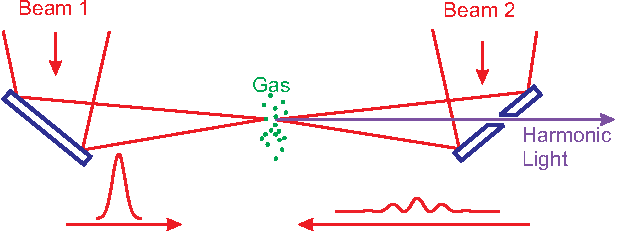
\includegraphics{Graphic1}}
    \caption[Setup for using counter-propagating light]{\label{fig:MirrorDiagram}
     A mirror with a hole is used to extract high-order harmonics generated in
     counter-propagating laser beams.}
\end{figure}







% Make the bibliography.
% Enter your references in the BibTex file "references.bib"
 \bibliography{references}

% Make the index
 \printindex

\end{document}
